%!TEX root = Main.tex
\appendix

\section{Scalability}
\label{sec:scalability}

\begin{figure}[t]
\centering
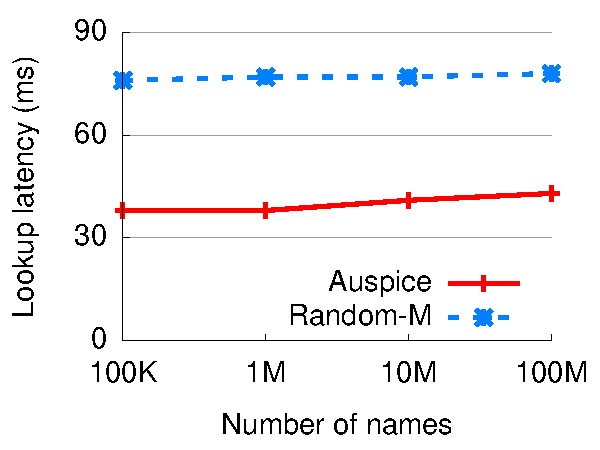
\includegraphics[scale=0.6]{graph/newgraphs/scalability.pdf}
\caption{\auspice's consistently gives close to 2$\times$ lower latencies for workloads with 100K-100M names.}
\vspace{-0.2in}
\label{fig:scalability}
\end{figure}

%How will \auspice\ perform at a scale of 10 billion mobile devices? 
To evaluate \auspice's key design traits at very high scales, we evaluate \auspice\ on workloads with 100K-100M device names.  We use a testbed of 200 Amazon EC2 instances, 100 each for nameservers and local nameservers respectively. We emulate wide-area latencies among servers as in the experiments in Section \ref{sec:lookup}. The experiment with a workload of 100M names included 1 billion requests with an equal number of lookups and updates sent over a 4 hour duration. Experiments with lesser number of names proportionally scale down the number of requests and the  duration.  
%As our focus is on evaluating the performance of \auspice's data plane, \auspice\ pre-computes the placement at the start of the experiment based on prior knowledge of the workload. Local name servers are also aware of the precomputed placement and they send requests directly to the active replicas in this experiment. Evaluating  \auspice's control plane performance at larger scales is part of our ongoing work.

Figure \ref{fig:scalability} shows that median lookup latency for Auspice and for \staticthree. We find that \auspice\ consistently gives close to 2$\times$ lower latency than \staticthree\ across all four workloads. 
\auspice's performance is consistent across workloads because its placement strategy ensures a similar distribution of load across name servers independent of the number of names in the workload.
Given that \auspice\ shows similar relative performance across 4 orders of magnitude of variation in the number of names, we expect these properties to persist at higher scales. Intuitively, this result is not surprising: the core of \auspice's replica placement engine is designed to make between M (the minimum required for fault-tolerance) and N (the total number of nameservers) replicas and use all available resources for intelligent replication. Group changes, although nontrivial in design, do not impose a high control overhead.



%This experiment shows that Auspice�s placement strategy gives consistent performance improvements over a static placement scheme on scaling the number of names in the workload. This finding suggests that \auspice's performance is likely to remain unchanged on further scaling the workload up a few orders of magnitude.



\eat {
\section{Scalability analysis}

In this subsection, we would like to quantify the scalability performance of \auspice. Assume there are $N$ names, for each name $i$ the lookup and update rates are $R_i$ and $W_i$ respectively. Then the lookup load is 
$$\sum_{i=1}^N R_i$$
and the update load is
$$\sum_{i=1}^N W_i$$
Since the total load on the system is control by a utilization threshold $\mu$ according to Eq. \ref{eq:mu}, then the control overhead required to maintain system consistency is:
$$\mu C - \sum_{i=1}^N R_i- \sum_{i=1}^N W_i$$
where $C$ is the total system capacity.

If we further use $n_i$ to denote the number of replicas for name $i$, and use $T$ to denote the  replication period, i.e., every time duration of $T$ the replication controllers recompute the active replicas for each name, then the overhead of recomputing active replicas is:
$$\sum_{i=1}^N \frac{ (M+6)n_i  + 6M-4}{T}$$
where $M$ is the minimum number of replicas for each name and we use 3 as its default value.

\eat {
Based on these equations, consider a back of the envelope calculation for a simple workload with $N=10^9$ names and 10,000 name servers. Each name has a rate of $R_i =0.001$ lookups and $W_i=0.001$ updates per second, and each name is replicated at $n_i=3$ servers. Each server has a capacity of 10,000 request per sec. Every $T=10^5$ sec, the system recomputes the active replicas for all names. 
Then the read load and write load each consumes 10\% of the total system capacity. The control overhead for maintaining system consistency is 70\% of the total capacity and the replication overhead is $4\%$.
}
\eat{
{\bf Latency:} Let's use $l_1$ and $l_2$ to denote the average lookup and update latencies across all clients and servers. Then
$$l_1 = a\ t + f(\mu c)$$
$$l_2 = b\ t + f(\mu c)$$
where $a$ and $b$ are constants to bound the maximum value of $r$. Therefore both lookup and update latencies remain the same as the number of name $N$ or the number of servers $S$ increases.
}
}

% by up to an order of magnitude.

%The name service enhances both mobility and security using self-certifying identifiers that on one hand cleanly separate identity from network location and on the other can be authenticated by any network entity without relying on a third-party. %We showed how a number of network services such as multi-homed traffic engineering, hierarchical routing, content retrieval, multicast, etc. can be implemented in an efficient and secure manner. 
%A key challenge that is addressed and is the focus of our experimental evaluation is the design of the distributed service to resolve identifiers to network locations. To this end, we presented \auspice, a service replica placement system that optimizes user-perceived latency by placing replicas of resolvers close to regions of high demand while respecting capacity and consistency constraints. \auspice\ is designed to be a flexible service replica placement engine that can be used to build services more general than name resolution. Our case studies with name resolution, social networking, and content distribution services show that \auspice\ yields significant improvements over state-of the-art alternatives for replicated service placement.

%\subsection{Placement optimization algorithms}
%\section{Optimization Formulation}
%\label{sec:mip}

%We present an optimization formulation that jointly optimizes  resolver placement and request redirection for a set of name records given the geo-distribution of their  requests, and the capacity of server deployments. The formulation optimizes for the overall user latency including network latency and server-load induced latency given a load-vs-response-time curve at each name server and network latency between users and name servers.


%In this section, we first present a {\em coordinated} placement algorithm based on an optimization approach and then present {\em uncoordinated} heuristic algorithms that moderately trade off latency or resource usage cost in exchange for a simpler and efficient implementation.

%\subsection{Model}

%Users requesting these services are located at distinct geographic regions. We partition the  geographic area spanning all the users, e.g. a continent or the entire world,  into non-overlapping geographic regions $U$.  Instead of calculating the latency to each user individually, we consider the average latency between users in a geographic region (called a \emph{user-group}) and each server location: $L_{ud}$ is the average latency between user-group  $u \in U$ and the deployment $d \in D$.


\eat {

\begin{table}[th]
\center
\begin{small}
\begin{tabular}{p{2.90in}}
\hline
\textbf{Parameters} \\

\end{tabular}
\begin{tabular}{p{0.25in}|p{2.5in}}
\hline
$U$ &  Set of geographic regions spanning all users \\ 
$D$ & Set of name servers\\
$S$ & Set of all name records\\
$C_d$ & Capacity of name server $d \in D$\\
$L_{ud} $ & Average latency between users in region $u \in U$ and name server location $d \in D$\\
$R_{us}$ & Lookup query rate of name record $s \in S$ from users in region $u \in U$\\ 
$W_s$ & Update query rate of name record $s \in S$\\
$B$ & Minimum number of resolvers of each name \\
$\alpha$ & Replication parameter for all name records\\
\hline
\end{tabular}

\begin{tabular}{p{2.9in}}
\hline
\textbf{Variables} \\
\end{tabular}
\begin{tabular}{p{0.25in}|p{2.5in}}
\hline
$x_{ds}$ & Binary variable indicating whether name record $s\in S$ is replicated at $d \in D$.\\
$y_{uds}$ & At location $d \in D$, lookup rate of users $u \in U$ for name record $s \in S$\\
\hline
\end{tabular}
\end{small}
\vspace{-0.1in}
\caption{\optimal\ parameters and variables}

\label{table:parameters}
\end{table}


All variables used in this formulation are described in Table \ref{table:parameters}. Let $D$ be the set of locations of name servers, and $C_d$ the total capacity of the name server at location $d \in D$.
Users requesting the name records are partitioned into distinct, geographically distributed network regions or user-groups $U$. The user-groups are assumed to be fine-grained enough so that the latency from any member of a user-group $u\in U$ to a name server $d$ is close to the average latency $L_{ud}$ from users in $u$ to $d$.

%We partition the  geographic area spanning all the users, e.g. a continent or the entire world,  into non-overlapping geographic regions $U$.  Instead of calculating the latency to each user individually, we consider the average latency between users in a geographic region (called a \emph{user-group}) and each server location: $L_{ud}$ is the average latency between user-group  $u \in U$ and the deployment $d \in D$.


% fault-tolerance and availability objectives.

The system decides the placement of resolvers and also decides to which resolver to redirect each user.  A user's request is assumed to be serviceable from any of the resolvers.  If a resolver of name record $s\in S$ is placed at location $d \in D$, the corresponding (binary) decision variable $x_{sd}$ takes the value 1,  otherwise $x_{sd}$ equals zero. The volume of requests from user-group $u \in U$ to the replica (if any) at location $d \in D$ of a service $s \in S$ is denoted by  $y_{uds}$,  a decision variable that takes values between $0$ and $r_{us}$.


\eat{
Our goal is to minimize the average latency between users and service replicas across all users in the system.  We ensure availability for all services by replicating each service at $B$ locations or more. 
}

%\subsection{Optimization formulation}
%\subsection{Optimization formulation}

Minimizing the average latency can be formulated as a mixed integer program. The following objective minimizes the aggregate latency across all users' requests. $M_d$ is the total server latency at name server $d\in D$. The first term and the second term denote the aggregate network and server latency respectively.
\begin{eqnarray}
\text{minimize:}\  \sum_{s \in S} \sum_{d \in D} \sum_{u \in U} L_{ud} \ x_{ds} \ y_{uds}  + \sum_{d \in D} M_d
\end{eqnarray}
The optimization must satisfy the constraints of the problem specified from Equation (5) to Equation (14).

All users' requests must be satisfied.
\begin{eqnarray}
\sum_{d \in D} {y_{uds}} = R_{us} \quad \forall u \in U, s \in S
\vspace{-0.1in}
\end{eqnarray}
The capacity at each name server must be greater than the total  request rate of users' and the update rate of  name records placed at that  location. The intermediate variable $t_d$ is the total request rate at name server $d \in D$.
\begin{eqnarray}
 \sum_{s \in S} \sum_{u \in U} y_{uds} + \sum_{s \in S} W_s\ x_{ds} = t_d   \leq C_d \quad \forall d \in D
\end{eqnarray}
Server utilization at $d \in D$ is $t_d / C_d$.  Server latency per request is defined as a function  of server utilization. The function $f$ is a piecewise convex linear function defined as $f(0) = 0$ and its derivatives.\vspace{-0.1in}
\begin{eqnarray}
f' (t_d / C_d)   =  \begin{cases}  r_1 & \text{if } 0 \leq t_d / C_d \leq u_1,  \notag \\
r_2 & \text{if } u_1 < t_d / C_d \leq u_2,  \notag \\
... & \notag \\
r_j & \text{if } u_{j - 1} < t_d / C_d \leq 1  \notag \end{cases}\\
\end{eqnarray}
%\vspace{-0.1in}
%Server latency increases with server utilization, so that $0 \leq r_1  < ... < r_j$. 
Essentially, the above equations transform a load vs. response time curve to a piecewise-linear, convex function, a technique that has also been in used in other domains \cite{fortz2000Internet} to make the optimization linear.
Let $M_d$ be the total server latency at location $d \in D$. $M_d$ is defined  by the following set of equations.
\begin{eqnarray}
v_0 = 0, u_0 = 0, u_j = 1\\
M_d \geq v_{i - 1} + r_i\ (t_d - u_{i -1} \ C_d) \quad \forall i \in \{1, 2, ..., j\}  \\
v_i = v_{i - 1} + r_i\ (u_i - u_{i - 1})\ C_d \quad \forall i \in \{1, 2, ..., j\} 
\end{eqnarray}
To ensure availability, each name record should be replicated at $B$ locations or more. \vspace{-0.05in}
\begin{eqnarray}
\sum_{d \in D} x_{ds} \geq B \quad \forall s \in S
\end{eqnarray}
A request can be served from a name server only if a resolved is placed at that name server. \vspace{-0.05in}
\begin{eqnarray}
y_{uds} \leq x_{ds} R_{us}\quad \forall u \in U, d \in D , s \in S
\end{eqnarray}
The next two equations constrain the values of each variable. \vspace{-0.05in}
\begin{eqnarray}
x_{ds} \in \{0, 1\} \quad \forall d \in D, s \in S
\end{eqnarray}
\vspace{-0.2in}
\begin{eqnarray}
0 \leq y_{uds} \leq R_{us} \quad \forall u \in U, d \in D , s \in S
\end{eqnarray}




%
%
%
%
%\eat{
%TODO:
%
%(1) remove the capacity constraint, formulate it as a LP problem and solve it using CPLEX tool
%
%(2) Either prove it is a NP hard, or show it is not
%
%(3) Constraints: bandwidth and computing/processing capacity at each server
%}
%
%\eat{
%\subsection{Server request processing delay}
%
%The above formulation does not optimize for request processing delay at the server, or \emph{server latency} for short. We describe an extension to the above formulation that optimizes for the overall user latency including network latency and server latency given a load-vs-response-time behavior for each service at each server is known.
%
%Let $t_d$ be the total request rate at location $d \in D$. From equation (3),
%\begin{eqnarray}
%t_d = \sum_{s \in S} \sum_{u \in U} y_{uds} + \sum_{s \in S} W_s\ x_{ds} 
%\end{eqnarray}
%The server utilization at $d \in D$ is $t_d / C_d$.  We define the server latency per request as a function  of server utilization. The function $f$ is shown below.
%\begin{eqnarray}
%f (t_d / C_d)   =  \begin{cases}  r_1 & \text{if } 0 \leq t_d / C_d \leq u_1,  \notag \\
%r_2 & \text{if } u_1 < t_d / C_d \leq u_2,  \notag \\
%... & \notag \\
%r_j & \text{if } u_{j - 1} < t_d / C_d \leq 1  \notag \end{cases}\\
%\end{eqnarray}
%Server latency increases with server utilization, so that $0 \leq r_1  < ... < r_j$. Essentially, the above transforms a load vs. response time curve to a piecewise-linear, convex function, a technique that has also been in used in other domains such as traffic engineering via optimization of OSPF weights \cite{fortz2000Internet} to make the optimization linear.
%
%Let $M_d$ be the total server latency at location $d \in D$. $M_d$ is defined  by the following set of equations.
%\begin{eqnarray}
%v_0 = 0, u_0 = 0, u_j = 1\\
%M_d \geq v_{i - 1} + r_i\ (t_d - u_{i -1} \ C_d) \quad \forall i \in \{1, 2, ..., j\}  \\
%v_i = v_{i - 1} + r_i\ (u_i - u_{i - 1})\ C_d \quad \forall i \in \{1, 2, ..., j\} 
%\end{eqnarray}
%
%Finally, we incorporate the total server latency $M_d$ at each location $d\in D$ into the objective function.
%
%
%\begin{eqnarray}
%\text{minimize:}\  \sum_{s \in S} \sum_{d \in D} \sum_{u \in U} L_{ud} \ x_{ds} \ y_{uds}  + \sum_{d \in D} M_d
%\end{eqnarray}
%}
%
%\eat{
%\subsection{Computational hardness}
%
%Mixed integer programs are generally computationally expensive to solve. We show that the service placement problem is NP-Complete via a reduction from the partition problem, with the proof deferred to Appendix \ref{appendix}. Thus, computing the optimal solution intrinsically demands a computationally expensive approach, motivating simpler heuristic placement algorithms.
%}
%%As the problem is  NP-Hard,  this problem can be solved optimally only via  computationally expensive approach such as the MIP presented above.
}